%% LaTeX-Beamer template for KIT design
%% by Erik Burger, Christian Hammer
%% title picture by Klaus Krogmann
%%
%% version 2.1
%%
%% mostly compatible to KIT corporate design v2.0
%% http://intranet.kit.edu/gestaltungsrichtlinien.php
%%
%% Problems, bugs and comments to
%% burger@kit.edu

\documentclass[18pt]{beamer}

%% SLIDE FORMAT

% use 'beamerthemekit' for standard 4:3 ratio
% for widescreen slides (16:9), use 'beamerthemekitwide'

\usepackage{templates/beamerthemekit}
% \usepackage{templates/beamerthemekitwide}

%% TITLE PICTURE

% if a custom picture is to be used on the title page, copy it into the 'logos'
% directory, in the line below, replace 'mypicture' with the 
% filename (without extension) and uncomment the following line
% (picture proportions: 63 : 20 for standard, 169 : 40 for wide
% *.eps format if you use latex+dvips+ps2pdf, 
% *.jpg/*.png/*.pdf if you use pdflatex)

\titleimage{KIT-Titel}

%% TITLE LOGO

% for a custom logo on the front page, copy your file into the 'logos'
% directory, insert the filename in the line below and uncomment it

\titlelogo{itiv-logo}

% (*.eps format if you use latex+dvips+ps2pdf,
% *.jpg/*.png/*.pdf if you use pdflatex)
  
%% TikZ INTEGRATION

% use these packages for PCM symbols and UML classes
% \usepackage{templates/tikzkit}
% \usepackage{templates/tikzuml}

% the presentation starts here

\title[Short title]{TikZ Tutorial}
\subtitle{KSETA Doktorandenworkshop 2014}
\author{Christian Amstutz, Tanja Harbaum, Ewa Holt}

\institute{}

% Bibliography

\usepackage[citestyle=authoryear,bibstyle=numeric,hyperref,backend=biber]{biblatex}
\addbibresource{templates/example.bib}
\bibhang1em

%*****************************************
% our packages
%*****************************************

\usepackage{listings}
\usepackage{graphicx}
\usepackage{amsmath,amssymb}
\usepackage{ifthen}


\usepackage{tikz}
\usetikzlibrary{positioning}
\usetikzlibrary{arrows}
\usetikzlibrary{shapes,snakes}
\usetikzlibrary{decorations.markings}
\usetikzlibrary{calc}

%*****************************************
% our definitions
%*****************************************

\lstdefinestyle{tikzstyle}{
  language=[LaTeX]tex,
  basicstyle=\scriptsize\ttfamily,
  keywordstyle=\bfseries\color{green!40!black},
  commentstyle=\itshape\color{purple!40!black},
  identifierstyle=\color{blue},
  stringstyle=\color{orange},
}

\lstnewenvironment{tikzcode}%
{\lstset{style=tikzstyle}}%
{}

\newcommand{\tikzcodefile}[1]{\lstinputlisting[style=tikzstyle]{#1}}


%*****************************************
%*****************************************
% the presentation
%*****************************************
%*****************************************


\begin{document}

% change the following line to "ngerman" for German style date and logos
\selectlanguage{english}


%*****************************************
%title page
%*****************************************

\begin{frame}
\titlepage
\end{frame}

%*****************************************
%table of contents
%*****************************************

\begin{frame}{Outline/Gliederung}
\tableofcontents
\end{frame}

%*****************************************
\section{TikZ}
\subsection{What is TikZ?}
\begin{frame}{What is TikZ?}

\begin{minipage}{0.70\textwidth}
\begin{itemize}
  \item Language for creating vector graphics in \LaTeX{}
  \item TikZ = \alert{T}ikZ \alert{i}st \alert{k}ein \alert{Z}eichenprogramm
\end{itemize}
\end{minipage}
\begin{minipage}{0.25\textwidth}
\pgfdeclarelayer{background}
\pgfdeclarelayer{foreground}
\pgfsetlayers{background,main,foreground}

\xdefinecolor{darkgreen}{RGB}{175, 193, 36}
\newcounter{cntShader}
\newcounter{cntRoot}
\setcounter{cntShader}{20}
\def\couleur{darkgreen}

\begin{tikzpicture}[scale=0.3,transform shape]
    \foreach \y in {86,38,15}{
        \setcounter{cntShader}{1}
        \coordinate (a) at (0,0);
        \coordinate (b) at (0:1);
        \foreach \x in {1,...,\y}{%
            \coordinate (c) at ($ (b)!1cm!270:(a) $);
            \begin{pgfonlayer}{background}
                \draw[fill=\couleur!\thecntShader] (a)--(b)--(c)--cycle;
            \end{pgfonlayer}
            \setcounter{cntRoot}{\x}
            \addtocounter{cntRoot}{1}
            \node[fill=white,draw,circle,inner sep=1pt] at (c)
                {$\sqrt{\thecntRoot}$};
            \coordinate (b) at (c);
            \pgfmathsetcounter{cntShader}{\thecntShader+4}
            \setcounter{cntShader}{\thecntShader}
       }
    }
    \node[fill=white,draw,circle,inner sep=1pt] at (0:1) {$\sqrt{1}$};
\end{tikzpicture}
\end{minipage}




\end{frame}
%*****************************************
\subsection{Why using TikZ?}
\begin{frame}{Why using TikZ?}
\begin{itemize}
  \item Single Design Among the Document
	\item \alert{One Design Flow}
	\item More versatile Image Scaling
	\item Math Environment within Graphics
	\item Automatic Graph Generation (Loops)
	\item combined with \LaTeX-Beamer class: graphics for presentations 
\end{itemize}

But be warned! It is not easy to learn.

\end{frame}

%*****************************************

\begin{frame}[fragile]{Scaling Effects}

\begin{tikzpicture}
\matrix[column sep=0.5cm] {
& \node {Raster Graphic (JPG)};
& \node {Vector Graphic (PDF)};
& \node {TikZ};
\\[2mm]
& \node {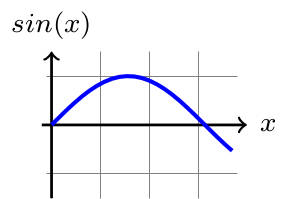
\includegraphics{tikz_bilder/sine_plot_standalone.jpg}};
& \node {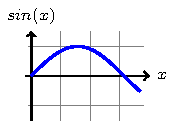
\includegraphics{tikz_bilder/sine_plot_standalone.pdf}};
& \node {
  \begin{tikzpicture}[domain=0:3.7, scale=0.5]
    \draw[very thin, color=gray] (-0.1,-1.5) grid (3.8,1.5);
  
  \draw[->, thick] (-0.2,0) -- (4,0) node[right] {\footnotesize $x$};
  \draw[->, thick] (0,-1.5) -- (0,1.5) node[above] {\footnotesize $sin(x)$};
  
  \draw[color=blue,very thick] plot (\x,{sin(\x r)});
  \end{tikzpicture}};
\\
& \node {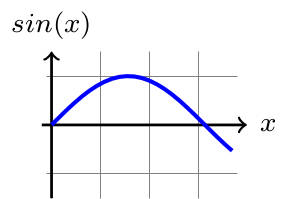
\includegraphics[clip, trim=0 15 37 0, scale=2]{tikz_bilder/sine_plot_standalone.jpg}};
& \node {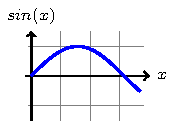
\includegraphics[clip, trim=0 15 37 0, scale=2]{tikz_bilder/sine_plot_standalone.pdf}};
& \node {
  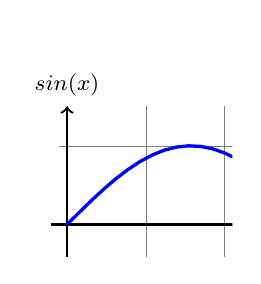
\begin{tikzpicture}[domain=0:3.7, scale=1]
  \clip (-0.5,-0.4) rectangle (2.1,2.5);
    \draw[very thin, color=gray] (-0.1,-1.5) grid (3.8,1.5);
  
  \draw[->, thick] (-0.2,0) -- (4,0) node[right] {\footnotesize $x$};
  \draw[->, thick] (0,-1.5) -- (0,1.5) node[above] {\footnotesize $sin(x)$};
  
  \draw[color=blue,very thick] plot (\x,{sin(\x r)});
  \end{tikzpicture}};
\\
};
\end{tikzpicture}

\end{frame}

%*****************************************

\begin{frame}{Math Environment}



% Define box and box title style
\tikzstyle{mybox} = [draw=red, fill=blue!20, very thick,
    rectangle, rounded corners, inner sep=10pt, inner ysep=20pt]
\tikzstyle{fancytitle} =[fill=red, text=white]

\begin{tikzpicture}[scale=0.7,transform shape]
\node [mybox] (box){%
    \begin{minipage}{0.50\textwidth}
        To calculate the horizontal position the kinematic differential
        equations are needed:
        \begin{align}
            \dot{n} &= u\cos\psi -v\sin\psi \\
            \dot{e} &= u\sin\psi + v\cos\psi
        \end{align}
        For small angles the following approximation can be used:
        \begin{align}
            \dot{n} &= u -v\delta_\psi \\
            \dot{e} &= u\delta_\psi + v
        \end{align}
    \end{minipage}
};
\node[fancytitle, right=10pt] at (box.north west) {A fancy title};
\node[fancytitle, rounded corners] at (box.east) {$\clubsuit$};
\end{tikzpicture}%
%
\tikzstyle{mybox} = [draw=blue, fill=green!20, very thick,
    rectangle, rounded corners, inner sep=10pt, inner ysep=20pt]
\tikzstyle{fancytitle} =[fill=blue, text=white, ellipse]
%
\begin{tikzpicture}[transform shape, rotate=10, baseline=-3.5cm,scale=0.7]
\node [mybox] (box) {%
    \begin{minipage}[t!]{0.5\textwidth}
        Fermat's Last Theorem states that
        \[
            x^n + y^n = z^n
        \]
        has no non-zero integer solutions for $x$, $y$ and $z$ when $n > 2$.
    \end{minipage}
    };
\node[fancytitle] at (box.north) {Fermat's Last Theorem};
\end{tikzpicture}

\end{frame}

%*****************************************

\begin{frame}{Loops}

\usetikzlibrary{matrix}
\usetikzlibrary{positioning,arrows}
\usetikzlibrary{through}
\usetikzlibrary{calc}
\usetikzlibrary{shapes,arrows}

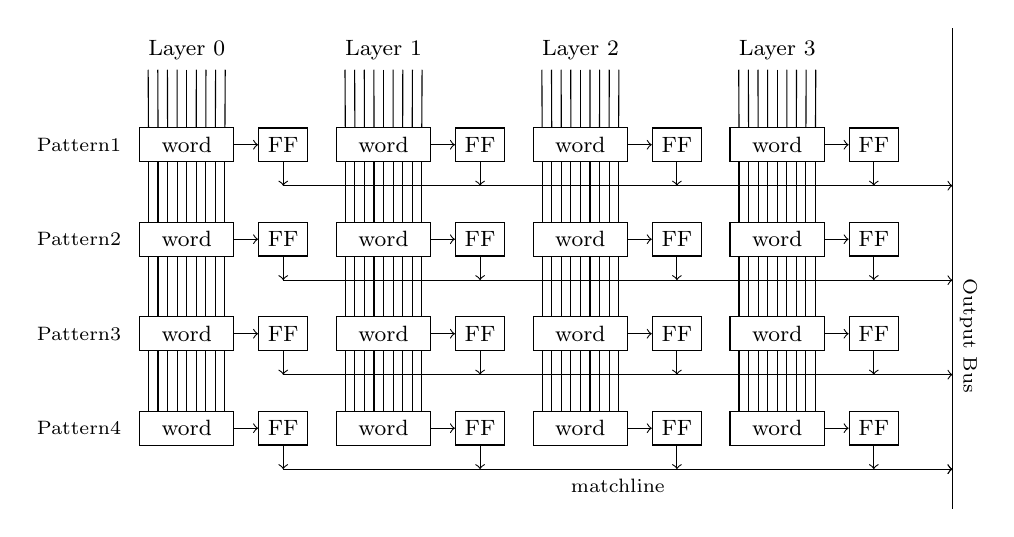
\begin{tikzpicture}

\tikzstyle{every node}=[rectangle, draw]
\tikzstyle{blank} = [coordinate]


    \foreach \x in {0,1,2,3} {
        \node[draw=none,minimum width=12mm] at (2.5*\x,0) (word\x0) {\footnotesize Layer \x};
}

 \foreach \y in {1,2,3,4} {
    \foreach \x in {0,1,2,3} {
        \node[minimum width=12mm] at (2.5*\x,-1.2*\y) (word\x\y) {\footnotesize word};
        \node[right=3mm of word\x\y] (ff\x\y){\footnotesize FF};
	\node[blank, below=3mm of ff\x\y](blank\x\y){};
	\draw[->](word\x\y) -- (ff\x\y);
	\draw[->](ff\x\y) -- (blank\x\y);
    }
\node[draw=none, left=1mm of word0\y](cell\y){\scriptsize Pattern\y};
\node[blank,right=10mm of blank3\y](blankbus\y){};
\draw[->](blank0\y) -- (blankbus\y);


}
\draw[->](blank04) -- (blankbus4) node[midway,below, draw=none]{\scriptsize matchline};

\node[blank,above=20mm of blankbus1](blankbus0){};
\node[blank,below=5mm of blankbus4](blankbus5){};
\draw[-](blankbus0) edge node [draw=none,right=2mm,rotate=-90] {\scriptsize Output Bus} (blankbus5);


 \foreach \y in {0,1,2,3} {
    \foreach \x in {0,1,2,3} {
\pgfmathtruncatemacro\next{\y+1}
\foreach \d in {0.1,0.2,0.3,0.4,0.5,0.6,0.7,0.8,0.9} {
\path (word\x\y.south west) -- (word\x\y.south east) coordinate[pos=\d] (a);
\path (word\x\next.north west) -- (word\x\next.north east) coordinate[pos=\d] (b);
\draw[] (a) -- (b);
}}
}

\end{tikzpicture}

\end{frame}

%*****************************************

\section{Commands}
\subsection{Setting Environment}
\begin{frame}[fragile]{Setting up the Environment in \LaTeX}

\begin{tikzcode}
\documentclass{standalone}

\usepackage{tikz}
\usetikzlibrary{ ... }

\begin{document}

\begin{tikzpicture}
  % TikZ commands go here  
\end{tikzpicture}

\end{document}
\end{tikzcode}

\end{frame}

%*****************************************
\subsection{Coordinates}
\begin{frame}{Coordinates}

\begin{columns}
  \begin{column}{0.5\textwidth}
  \end{column}
  \begin{column}{0.5\textwidth}
  \end{column}
\end{columns}

\end{frame}

%*****************************************
\subsection{draw Command}
\begin{frame}[fragile]{The \texttt{\textbackslash draw} Command}

\begin{columns}
  \begin{column}{0.5\textwidth}
  \begin{tikzcode}
  \draw (0,0) -- (1,1);
  \draw[->] (1,1) -- (1,0);
  \draw (0,0) rectangle (1,1);
  \draw (1,1) circle [radius=0.5];
  \end{tikzcode}
  \end{column}
  \begin{column}{0.5\textwidth}
  \begin{tikzpicture}
    \draw (0,0) -- (1,1);
  \end{tikzpicture}\\
  \begin{tikzpicture}
    \draw[->] (1,1) -- (1,0);
  \end{tikzpicture}\\
  
\begin{tikzpicture}
    \draw (0,0) rectangle (1,1);
  \end{tikzpicture}\\
  
\begin{tikzpicture}
    \draw (1,1) circle [radius=0.5];
  \end{tikzpicture}
  \end{column}
\end{columns}

\end{frame}

%*****************************************
\subsection{node Command}
\begin{frame}[fragile]{The \texttt{\textbackslash node} Command}

A node is typically a rectangle or circle or another simple shape with some text on it

\begin{minipage}{0.80\textwidth}
\begin{tikzcode}
\node[rectangle,fill=green](rect) {Rectangle};
\end{tikzcode}
\end{minipage}
\begin{minipage}{0.15\textwidth}
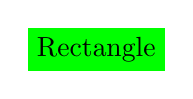
\begin{tikzpicture}
  \node[rectangle,fill=green](rect) {Rectangle};
\end{tikzpicture}
\end{minipage}

\vspace{1em}


Node positioning

\begin{minipage}{0.85\textwidth}
\begin{tikzcode}
\node[rectangle,fill=green](rect){Rectangle};
\node[circle,fill=purple,below=of rect](circ){Circle};
\end{tikzcode}
\end{minipage}
\begin{minipage}{0.1\textwidth}
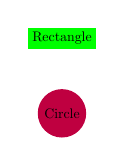
\begin{tikzpicture}[scale=0.5,transform shape]
  \node[rectangle,fill=green](rect) {Rectangle};
 \node[circle,fill=purple, below = of rect] (circ) {Circle};
\end{tikzpicture}
\end{minipage}

Connect nodes with lines

\begin{minipage}{0.85\textwidth}
\begin{tikzcode}
\node[rectangle,fill=green](rect){Rectangle};
\node[circle,fill=purple,below=of rect](circ){Circle};
\draw[->] (rect) -- (circ);
\end{tikzcode}
\end{minipage}
\begin{minipage}{0.1\textwidth}
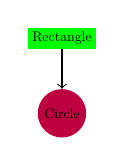
\begin{tikzpicture}[scale=0.5,transform shape]
\node[rectangle,fill=green](rect){Rectangle};
\node[circle,fill=purple,below=of rect](circ){Circle};
\draw[->] (rect) -- (circ);
\end{tikzpicture}
\end{minipage}

\end{frame}

%*****************************************
\subsection{style Definition}
\begin{frame}[fragile]{Style Definitions}

Styles are defined by \texttt{[]} behind a command

\begin{minipage}{0.80\textwidth}
\begin{tikzcode}
\draw[red, very thick, dashed] (0,0) -- (1,0.1);
\end{tikzcode}
\end{minipage}
\begin{minipage}{0.15\textwidth}
\begin{tikzpicture}
  \draw[red, very thick, dashed] (0,0,) -- (1,0.1);
\end{tikzpicture}
\end{minipage}

\vspace{1em}

Styles can be named and defined locally or globally

\begin{tikzcode}
\tikzset{my style/.style={tikz options}}
\tikzstyle{my style}=[tikz options]       % deprecated
\end{tikzcode}

\vspace{1em}

example

\begin{minipage}{0.9\textwidth}
\begin{tikzcode}
\tikzset{my dot/.style={blue, fill=green, thick}}
\draw[my dot] (0,0) circle [radius=0.1];
\draw[my dot] (0.1,0.4) circle [radius=0.1];
\draw[my dot, fill=red] (0.3,0.1) circle [radius=0.1];
\end{tikzcode}
\end{minipage}
\begin{minipage}{0.05\textwidth}
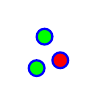
\begin{tikzpicture}
\tikzset{my dot/.style={blue, fill=green, thick}}
\draw[my dot] (0,0) circle [radius=0.1];
\draw[my dot] (0.1,0.4) circle [radius=0.1];
\draw[my dot, fill=red] (0.3,0.1) circle [radius=0.1];
\end{tikzpicture}
\end{minipage}

\end{frame}

%*****************************************
  
\section{Exercises}
\subsection{UML Activity Diagram}
\begin{frame}{Exercise 1: UML Activity Diagram}

\note{

}

\usetikzlibrary{shapes}
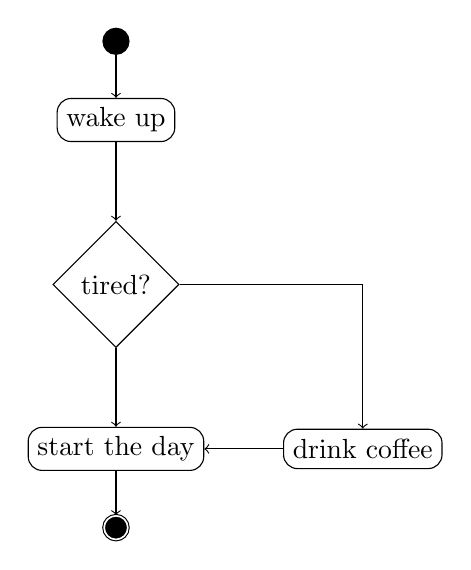
\begin{tikzpicture}
  
\tikzstyle{activity}=[rectangle,minimum width=1cm,minimum height=0.5cm, rounded corners=5pt, draw]
\tikzstyle{start}=[circle,minimum width=0.3cm,minimum height=0.3cm, draw, fill]
\tikzstyle{end}=[draw,double=white, circle, inner sep=1pt,minimum width=0.3cm,minimum height=0.3cm, fill]
\tikzstyle{decision}=[diamond,minimum width=1cm,minimum height=1cm, draw]
\tikzstyle{blank} = [coordinate]%[rectangle, text width=0em, text centered, rounded corners, minimum height=0em]

\node[start] (start) {};
\node[activity, below of = start] (action1) {wake up};
\node[decision,below = of  action1](decision1){tired?};
\node[activity, below = of  decision1] (action2) {start the day};
\node[activity, right = of action2] (action3) {drink coffee};
\node[end,below of = action2](end){};


\draw[->](start) -- (action1);
\draw[->](action1) -- (decision1);
\draw[->](decision1) -- (action2);
\draw[->](decision1) -| (action3);
\draw[->](action3) -- (action2);
\draw[->](action2) -- (end);

\end{tikzpicture}


\end{frame}

%*****************************************  


\begin{frame}[fragile]{Exercise 1: UML Activity Diagram}


\begin{tikzcode}
\tikzset{start/.style	={circle,minimum width=0.3cm,
                       minimum height=0.3cm, draw, fill}}
\node[start] (start) {};
\end{tikzcode}

\vspace{1em}


\begin{tikzpicture}[scale=0.7,transform shape]
\tikzset{start/.style={circle,minimum width=0.3cm,minimum height=0.3cm, draw, fill}}
\node[start] (start) {};
\end{tikzpicture}


\end{frame}

%*****************************************
  


\begin{frame}[fragile]{Exercise 1: UML Activity Diagram}


\begin{tikzcode}
\tikzset{activity/.style={rectangle,minimum width=1cm,
                 minimum height=0.5cm, rounded corners=5pt, draw}}
\node[activity, below of = start] (action1) {wake up};
\end{tikzcode}

\vspace{1em}

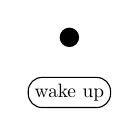
\begin{tikzpicture}[scale=0.7,transform shape]
\tikzset{activity/.style={rectangle,minimum width=1cm,minimum height=0.5cm, rounded corners=5pt, draw}}
\tikzset{start/.style={circle,minimum width=0.3cm,minimum height=0.3cm, draw, fill}}
\node[start] (start) {};
\node[activity, below of = start] (action1) {wake up};
\end{tikzpicture}


\end{frame}

%*****************************************
  


\begin{frame}[fragile]{Exercise 1: UML Activity Diagram}


\begin{tikzcode}
\tikzset{decision/.style={diamond,minimum width=1cm,
                         minimum height=1cm, draw}}
\node[decision,below = of  action1](decision1){tired?};
\end{tikzcode}

\vspace{1em}

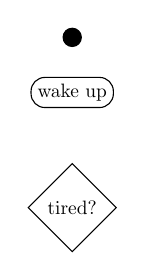
\begin{tikzpicture}[scale=0.7,transform shape]
\tikzset{activity/.style={rectangle,minimum width=1cm,minimum height=0.5cm, rounded corners=5pt, draw}}
\tikzset{decision/.style={diamond,minimum width=1cm,minimum height=1cm, draw}}
\tikzset{start/.style={circle,minimum width=0.3cm,minimum height=0.3cm, draw, fill}}
\node[start] (start) {};
\node[activity, below of = start] (action1) {wake up};
\node[decision,below = of  action1](decision1){tired?};
\end{tikzpicture}


\end{frame}

%*****************************************
  


\begin{frame}[fragile]{Exercise 1: UML Activity Diagram}


\begin{tikzcode}
\node[activity, below = of decision1] (action2) {start the day};
\node[activity, right = of action2] (action3) {drink coffee};
\end{tikzcode}

\vspace{1em}

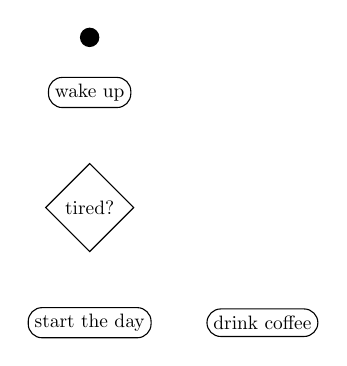
\begin{tikzpicture}[scale=0.7,transform shape]
\tikzset{activity/.style={rectangle,minimum width=1cm,minimum height=0.5cm, rounded corners=5pt, draw}}
\tikzset{decision/.style={diamond,minimum width=1cm,minimum height=1cm, draw}}
\tikzset{start/.style={circle,minimum width=0.3cm,minimum height=0.3cm, draw, fill}}
\node[start] (start) {};
\node[activity, below of = start] (action1) {wake up};
\node[decision,below = of  action1](decision1){tired?};
\node[activity, below = of  decision1] (action2) {start the day};
\node[activity, right = of action2] (action3) {drink coffee};
\end{tikzpicture}


\end{frame}

%*****************************************
  


\begin{frame}[fragile]{Exercise 1: UML Activity Diagram}


\begin{tikzcode}
\tikzset{end/.style={draw,double=white, circle,
               inner sep=1pt,minimum width=0.3cm,minimum height=0.3cm, fill}}
\node[end,below of = action2](end){};
\end{tikzcode}

\vspace{1em}

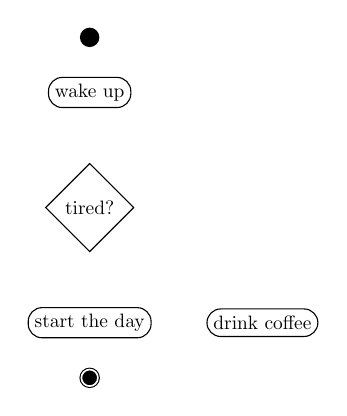
\begin{tikzpicture}[scale=0.7,transform shape]
\tikzset{activity/.style={rectangle,minimum width=1cm,minimum height=0.5cm, rounded corners=5pt, draw}}
\tikzset{decision/.style={diamond,minimum width=1cm,minimum height=1cm, draw}}
\tikzset{start/.style={circle,minimum width=0.3cm,minimum height=0.3cm, draw, fill}}
\tikzset{end/.style={draw,double=white, circle, inner sep=1pt,minimum width=0.3cm,minimum height=0.3cm, fill}}
\node[start] (start) {};
\node[activity, below of = start] (action1) {wake up};
\node[decision,below = of  action1](decision1){tired?};
\node[activity, below = of  decision1] (action2) {start the day};
\node[activity, right = of action2] (action3) {drink coffee};
\node[end,below of = action2](end){};
\end{tikzpicture}


\end{frame}

%*****************************************
  

\begin{frame}[fragile]{Exercise 1: UML Activity Diagram}


\begin{tikzcode}
\draw[->](start) -- (action1);
\draw[->](action1) -- (decision1);
\draw[->](action3) -- (action2);
\draw[->](action2) -- (end);
\end{tikzcode}

\vspace{1em}

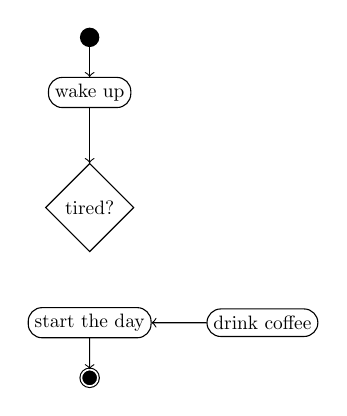
\begin{tikzpicture}[scale=0.7,transform shape]
\tikzset{activity/.style={rectangle,minimum width=1cm,minimum height=0.5cm, rounded corners=5pt, draw}}
\tikzset{decision/.style={diamond,minimum width=1cm,minimum height=1cm, draw}}
\tikzset{start/.style={circle,minimum width=0.3cm,minimum height=0.3cm, draw, fill}}
\tikzset{end/.style={draw,double=white, circle, inner sep=1pt,minimum width=0.3cm,minimum height=0.3cm, fill}}
\node[start] (start) {};
\node[activity, below of = start] (action1) {wake up};
\node[decision,below = of  action1](decision1){tired?};
\node[activity, below = of  decision1] (action2) {start the day};
\node[activity, right = of action2] (action3) {drink coffee};
\node[end,below of = action2](end){};
\draw[->](start) -- (action1);
\draw[->](action1) -- (decision1);
\draw[->](action3) -- (action2);
\draw[->](action2) -- (end);
\end{tikzpicture}


\end{frame}

%*****************************************
  

\begin{frame}[fragile]{Exercise 1: UML Activity Diagram}


\begin{tikzcode}
\draw[->](decision1) -- node [left,very near start]{no} (action2);
\draw[->](decision1) -| node [above,very near start]{yes} (action3) ;
\end{tikzcode}

\vspace{1em}

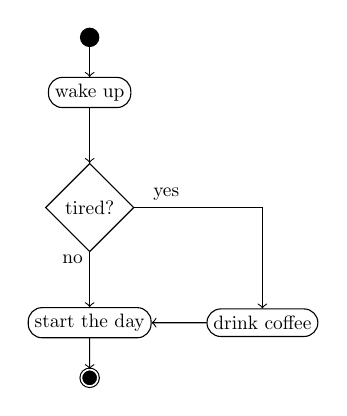
\begin{tikzpicture}[scale=0.7,transform shape]
\tikzset{activity/.style={rectangle,minimum width=1cm,minimum height=0.5cm, rounded corners=5pt, draw}}
\tikzset{decision/.style={diamond,minimum width=1cm,minimum height=1cm, draw}}
\tikzset{start/.style={circle,minimum width=0.3cm,minimum height=0.3cm, draw, fill}}
\tikzset{end/.style={draw,double=white, circle, inner sep=1pt,minimum width=0.3cm,minimum height=0.3cm, fill}}
\node[start] (start) {};
\node[activity, below of = start] (action1) {wake up};
\node[decision,below = of  action1](decision1){tired?};
\node[activity, below = of  decision1] (action2) {start the day};
\node[activity, right = of action2] (action3) {drink coffee};
\node[end,below of = action2](end){};
\draw[->](start) -- (action1);
\draw[->](action1) -- (decision1);
\draw[->](action3) -- (action2);
\draw[->](action2) -- (end);
\draw[->](decision1) -- node [left,very near start]{no} (action2);
\draw[->](decision1) -| node [above,very near start]{yes} (action3) ;
\end{tikzpicture}

\end{frame}
%*****************************************

\begin{frame}[fragile, allowframebreaks]{Exercise 1:\\ UML Activity Diagram - Solution}

\tikzcodefile{tikz_bilder/exercise_uml.tex}

\end{frame}

%*****************************************



\subsection{Feynman-Diagram}

\begin{frame}{Exercise 1: Feynman Diagram}

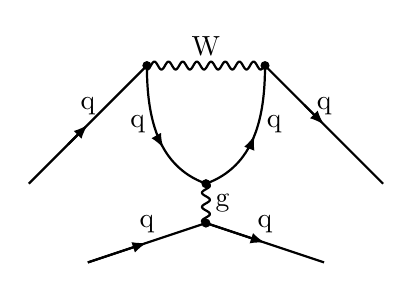
\begin{tikzpicture}[xscale=0.5, yscale=0.5]
    \draw[thick] (0.5,5) -- (3.5,8);
    \draw[-latex,thick] (1.5,6) -- (2,6.5);
    \node[above] at (2,6.5){q};
    \draw [fill] (3.5,8) circle [radius=0.1];
    \draw [domain=3.5:6.5, thick, samples=200] plot (\x,{8+0.1*sin(1000*\x)});
    \node[above] at (5,8){W};
    \draw [fill] (6.5,8) circle [radius=0.1];
    \draw[thick] (6.5,8) -- (9.5,5);
    \draw[-latex,thick] (7.5,7) -- (8,6.5);
    \node[above] at (8,6.5){q};
    \draw[thick,decoration={markings, mark=at position 0.6 with {\arrow{latex}}},postaction={decorate}] 
    		(3.5,8) to [out=-90, in=160] (5,5);
    	\node[left] at (3.7,6.5){q};
    	\draw[thick,decoration={markings, mark=at position 0.5 with {\arrow{latex}}},postaction={decorate}] 
    		(5,5) to [out=20, in=270] (6.5,8);
    	\node[right] at (6.3,6.5){q};
    \draw [fill] (5,5) circle [radius=0.1];
    \draw [domain=4:5, thick, samples=200, rotate=90] plot (\x,{-5+0.1*sin(1000*\x)});
    \node[right] at (5,4.5){g};
    \draw [fill] (5,4) circle [radius=0.1];
    \draw[thick] (2,3) -- (5,4);
    \draw[-latex,thick] (2,3) -- (3.5,3.5);
	\node[above] at (3.5,3.5){q};
    \draw[thick] (5,4) -- (8,3);
    \draw[-latex,thick] (5,4) -- (6.5,3.5);
    \node[above] at (6.5,3.5){q};
\end{tikzpicture}
  
\end{frame}
  


%*****************************************

\subsection{Plotting Data}

\begin{frame}{Exercise 3: Plot}

\note{
  - Using plots from different tools, these would look differently
  - Formulas in plots
  - Line width adaptation
  - Scaling effects
  - nicer view
  
  more information: Chapter 19 of the official documentation
}

\begin{tikzpicture}[domain=0.2:6]
  
  \draw[->, >=stealth'] (-0.2,0) -- (7,0) node[right] {$x$};
  \draw[->, >=stealth'] (0,-0.2) -- (0,6) node[above] {$f(x)$};
  
  \foreach \x in {0.5,1,1.5,2,2.5,3,3.5,4,4.5,5,5.5,6,6.5}
    \draw (\x,2pt) -- (\x,-3pt);
  \foreach \x in {0,1,2,3,4,5,6}
    \node at (\x,-6pt) [anchor=north] {\footnotesize $\x$};    
  \foreach \y/\ytext in {0.5,1,1.5,2,2.5,3,3.5,4,4.5,5,5.5}
    \draw (2pt,\y) -- (-3pt,\y cm);
  \foreach \y/\ytext in {0,1,2,3,4,5}
    \node at (-6pt,\y) [anchor=east] {\footnotesize $\ytext$};
  
  \draw plot[only marks, mark=x, mark options={kit-blue100, thick}]
      file {tikz_bilder/measurement.dat};
  \draw[color=kit-green100] plot[smooth] (\x, {1+pow((1/3)*\x, 2)})
      node[right, xshift=6mm] {$f(x) = 1+\frac{1}{3}x^{2}$};

\end{tikzpicture}


\end{frame}

%*****************************************

\begin{frame}[fragile, allowframebreaks]{Exercise 1: Feynman Diagram}

\tikzcodefile{tikz_bilder/exercise_feynman.tex}
  
\end{frame}



%*****************************************

\begin{frame}[fragile]{Exercise 3: Plot - Solution}

\tikzcodefile{tikz_bilder/exercise_plot.tex}

\end{frame}


%*****************************************
\section{Fancy Examples}
\subsection{Polarizing Microscope}
\begin{frame}{Fancy Examples - Polarizing Microscope}
% Polarizing microscope
% Author: Cyril Langlois
% This TikZ code sketches the light behavior during its travel in a polarizing
% petrographic microscope when a birefringent crystal thin section is inserted
% between the polarizing devices.
% 
% The goal was to correctly show the vectorial relationships between light
% electric fields during its travel through the first polaroid, the mineral
% section and the second polaroid.

\usetikzlibrary{arrows}

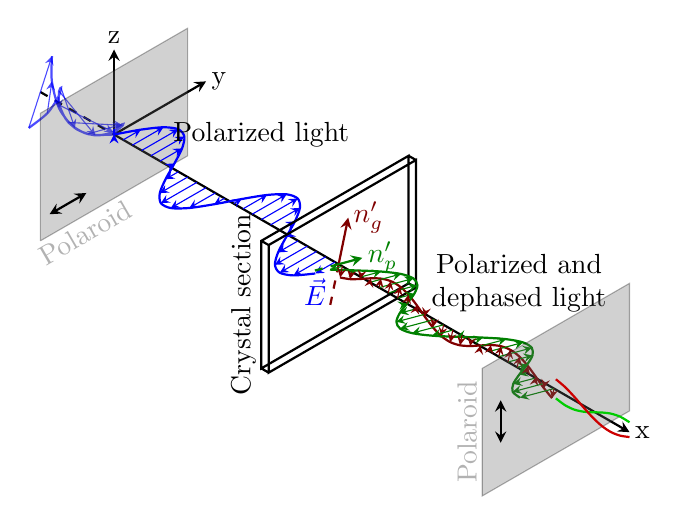
\begin{tikzpicture}[x={(0.866cm,-0.5cm)}, y={(0.866cm,0.5cm)}, z={(0cm,1cm)}, scale=0.54,
    %Option for nice arrows
    >=stealth, %
    inner sep=0pt, outer sep=2pt,%
    axis/.style={thick,->},
    wave/.style={thick,color=#1,smooth},
    polaroid/.style={fill=black!60!white, opacity=0.3},
]
    % Colors
    \colorlet{darkgreen}{green!50!black}
    \colorlet{lightgreen}{green!80!black}
    \colorlet{darkred}{red!50!black}
    \colorlet{lightred}{red!80!black}

    % Frame
    \coordinate (O) at (0, 0, 0);
    \draw[axis] (O) -- +(14, 0,   0) node [right] {x};
    \draw[axis] (O) -- +(0,  2.5, 0) node [right] {y};
    \draw[axis] (O) -- +(0,  0,   2) node [above] {z};

    \draw[thick,dashed] (-2,0,0) -- (O);

    % monochromatic incident light with electric field
    \draw[wave=blue, opacity=0.7, variable=\x, samples at={-2,-1.75,...,0}]
        plot (\x, { cos(1.0*\x r)*sin(2.0*\x r)}, { sin(1.0*\x r)*sin(2.0*\x r)})
        plot (\x, {-cos(1.0*\x r)*sin(2.0*\x r)}, {-sin(1.0*\x r)*sin(2.0*\x r)});

    \foreach \x in{-2,-1.75,...,0}{
        \draw[color=blue, opacity=0.7,->]
            (\x,0,0) -- (\x, { cos(1.0*\x r)*sin(2.0*\x r)}, { sin(1.0*\x r)*sin(2.0*\x r)})
            (\x,0,0) -- (\x, {-cos(1.0*\x r)*sin(2.0*\x r)}, {-sin(1.0*\x r)*sin(2.0*\x r)});
    }

    \filldraw[polaroid] (0,-2,-1.5) -- (0,-2,1.5) -- (0,2,1.5) -- (0,2,-1.5) -- (0,-2,-1.5)
        node[below, sloped, near end]{Polaroid};%

    %Direction of polarization
    \draw[thick,<->] (0,-1.75,-1) -- (0,-0.75,-1);

    % Electric field vectors
    \draw[wave=blue, variable=\x,samples at={0,0.25,...,6}]
        plot (\x,{sin(2*\x r)},0)node[anchor=north]{$\vec{E}$};

    %Polarized light between polaroid and thin section
    \foreach \x in{0, 0.25,...,6}
        \draw[color=blue,->] (\x,0,0) -- (\x,{sin(2*\x r)},0);

    \draw (3,1,1) node [text width=2.5cm, text centered]{Polarized light};

    %Crystal thin section
    \begin{scope}[thick]
        \draw (6,-2,-1.5) -- (6,-2,1.5) node [above, sloped, midway]{Crystal section}
                -- (6, 2, 1.5) -- (6, 2, -1.5) -- cycle % First face
            (6,  -2, -1.5) -- (6.2, -2,-1.5)
            (6,   2, -1.5) -- (6.2,  2,-1.5)
            (6,  -2,  1.5) -- (6.2, -2, 1.5)
            (6,   2,  1.5) -- (6.2,  2, 1.5)
            (6.2,-2, -1.5) -- (6.2, -2, 1.5) -- (6.2, 2, 1.5) 
                -- (6.2, 2, -1.5) -- cycle; % Second face

        %Optical indices
        \draw[darkred, ->]       (6.1, 0, 0) -- (6.1, 0.26,  0.966) node [right] {$n_{g}'$}; % index 1
        \draw[darkred, dashed]   (6.1, 0, 0) -- (6.1,-0.26, -0.966); % index 1
        \draw[darkgreen, ->]     (6.1, 0, 0) -- (6.1, 0.644,-0.173) node [right] {$n_{p}'$}; % index 2
        \draw[darkgreen, dashed] (6.1, 0, 0) -- (6.1,-0.644, 0.173); % index 2
    \end{scope}

    %Rays leaving thin section
    \draw[wave=darkred,   variable=\x, samples at={6.2,6.45,...,12}] 
        plot (\x, {0.26*0.26*sin(2*(\x-0.5) r)},  {0.966*0.26*sin(2*(\x-0.5) r)});  %n'g-oriented ray
    \draw[wave=darkgreen, variable=\x, samples at={6.2,6.45,...,12}]
        plot (\x, {0.966*0.966*sin(2*(\x-0.1) r)},{-0.26*0.966*sin(2*(\x-0.1) r)}); %n'p-oriented ray
    \draw (10,1,1) node [text width=2.5cm, text centered] {Polarized and dephased light};

    \foreach \x in{6.2,6.45,...,12} {
        \draw[color=darkgreen, ->] (\x, 0, 0) --
            (\x, {0.966*0.966*sin(2*(\x-0.1) r)}, {-0.26*0.966*sin(2*(\x-0.1) r)});
        \draw[color=darkred,   ->] (\x, 0, 0) --
            (\x, {0.26*0.26*sin(2*(\x-0.5) r)}, {0.966*0.26*sin(2*(\x-0.5) r)});
    }

    %Second polarization
    \draw[polaroid]   (12, -2,  -1.5) -- (12, -2,   1.5)  %Polarizing filter
        node [above, sloped,midway] {Polaroid} -- (12, 2, 1.5) -- (12, 2, -1.5) -- cycle;
    \draw[thick, <->] (12, -1.5,-0.5) -- (12, -1.5, 0.5); %Polarization direction

    %Light leaving the second polaroid
    \draw[wave=lightgreen,variable=\x, samples at={12, 12.25,..., 14}]
        plot (\x,{0}, {0.966*0.966*0.26*sin(2*(\x-0.5) r)}); %n'g polarized ray
    \draw[wave=lightred,  variable=\x, samples at={12, 12.25,..., 14}]
        plot (\x,{0}, {-0.26*0.966*sin(2*(\x-0.1) r)});      %n'p polarized ray


\end{tikzpicture}
\end{frame}

%*****************************************
\subsection{Mind Map}
\begin{frame}{Fancy Examples - Mind Map}
\usetikzlibrary{mindmap,trees}

\begin{tikzpicture}[scale=0.5,transform shape]
  \path[mindmap,concept color=black,text=white]
    node[concept] {Computer Science}
    [clockwise from=0]
    child[concept color=green!50!black] {
      node[concept] {practical}
      [clockwise from=90]
      child { node[concept] {algorithms} }
      child { node[concept] {data structures} }
      child { node[concept] {pro\-gramming languages} }
      child { node[concept] {software engineer\-ing} }
    }  
    child[concept color=blue] {
      node[concept] {applied}
      [clockwise from=-30]
      child { node[concept] {databases} }
      child { node[concept] {WWW} }
    }
    child[concept color=red] { node[concept] {technical} }
    child[concept color=orange] { node[concept] {theoretical} };
\end{tikzpicture}
\end{frame}

%*****************************************
\section{}
\begin{frame}{More information}

Website with nice TikZ examples:\\
\href{http://www.texample.net/tikz/examples}%
  {http://www.texample.net/tikz/examples}
\vspace{1em}
A very minimal introduction to TikZ - A good short introduction\\
\href{http://cremeronline.com/LaTeX/minimaltikz.pdf}%
  {http://cremeronline.com/LaTeX/minimaltikz.pdf}
\vspace{1em}
TikZ \ PGF Manual (Version 3.0) - great resource written in clear, comprehensible language\\
\href{http://mirrors.ctan.org/graphics/pgf/base/doc/pgfmanual.pdf}%
  {http://mirrors.ctan.org/graphics/pgf/base/doc/pgfmanual.pdf} (Version 3.0)
\vspace{1em}
TikZ Cheat Sheet - short cheatsheet far from being complete\\
\href{http://home.snc.edu/andershendrickson/tex/TikZcheatsheet.pdf}%
  {http://home.snc.edu/andershendrickson/tex/TikZcheatsheet.pdf}

\end{frame}
%*****************************************

\begin{frame}

\vspace{1cm}  
\begin{center}
  \begin{Huge}Thank you for your attention\end{Huge}
\end{center}
  
\end{frame}

%*****************************************
\appendix
%\beginbackup

%\begin{frame}[allowframebreaks]{References}
%\printbibliography
%\end{frame}

%\backupend

\end{document}
